\documentclass{beamer}

\usepackage[utf8]{inputenc}
\usepackage[T1]{fontenc}
\usepackage{lmodern}
\usepackage{microtype}

\usepackage{color}
\usepackage{tikz}

\usepackage{amssymb}
\usepackage{amsmath}

\addtobeamertemplate{navigation symbols}{}{%
    \usebeamerfont{footline}%
    \usebeamercolor[fg]{footline}%
    \hspace{1em}%
    \insertframenumber
}


\begin{document}
\title{Strengthening memory safety in Rust:\\
Exploring CHERI capabilities for a safe language}
\author{Nicholas Sim}
\date{June 21, 2019}

\frame{\titlepage}


\begin{frame}
\frametitle{Why memory safety is important}

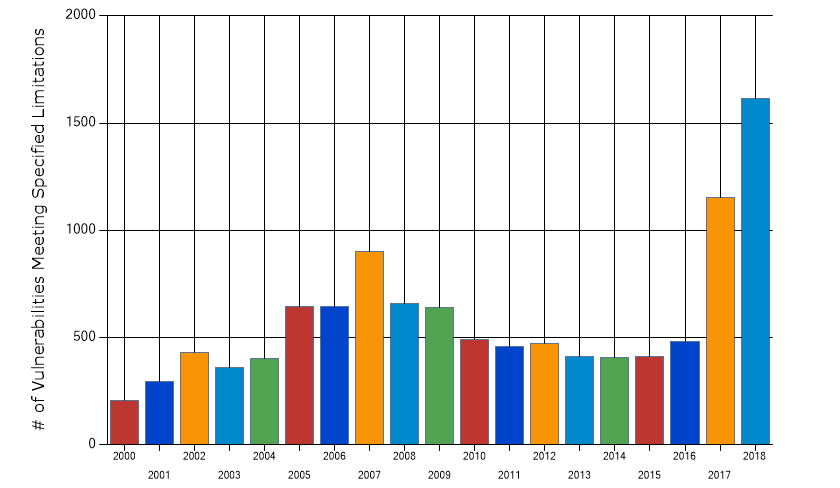
\includegraphics[width=\textwidth]{graph-overflow.png}
\begin{itemize}
    \item Buffer overflows \emph{still} on the rise [fig.: NIST NVD]
\end{itemize}
\end{frame}


\begin{frame}
\frametitle{CHERI: capablity architecture}

\begin{itemize}
    \item An instruction set architecture, extends RISC
    \item Offers hardware capabilities: unforgeable tokens for pointers
    \item Protects memory from unauthorised access
    \item MORE
    \item Under development here
    \item Mainly studied under C: capabilities known to be effective for
    unsafe languages
    \item Do safe languages benefit more? Less?
\end{itemize}
\end{frame}


\begin{frame}
\frametitle{Rust: safe language}

\begin{itemize}
    \item New programming language (c.\ 2012)
    \item Rust's models ``guarantee memory safety'' (big claim!)
    \item Boasts of performance \emph{and} memory safety
    \item Recognises that C is too complex, too much undefined behaviour\footnote{viz.\ Memarian et al.\ 2016}
    \item Split into \emph{Safe}, \emph{Unsafe} Rust
    \item For safety and power respectively
\end{itemize}
\end{frame}


\begin{frame}
\frametitle{Rust: safe language?}

\begin{itemize}
    \item 7 vulnerabilities and counting in standard library + compiler
    \item 5 fully prevented by capabilities!
    \item Array bounds checks: irrelevant with capabilities
    \item Possible to optimise checks?
    \item Other benefits? (write)
\end{itemize}
\end{frame}


\begin{frame}
\frametitle{Contributions}

\begin{itemize}
    \item CHERI support in the Rust compiler
    \item Analysis of past vulnerabilities
    \item Demonstration that capabilities mitigate them
    \item Evaluation of techniques to optimise capability usage
    \item Methods to use CHERI features e.g.\ sealing improve Rust guarantees
    \item How capability interactions with the language (pointer width,
    undefined behaviour)
\end{itemize}
\end{frame}


\begin{frame}
\frametitle{Evaluation: Improving Rust safety}

\begin{itemize}
    \item (I plan to discuss sealing and the hybrid ABI, especially
    selectively using capabilities and performance vs C. 1--2 slides.)
    \item In particular I don't plan to mention the microbenchmarks in
    this section
\end{itemize}
\end{frame}


\begin{frame}
\frametitle{Evaluation: in the report}

\begin{itemize}
    \item Rust semantics provide guarantees under CHERI that C cannot
    \item Eliminate bounds checks, leaks, use-after-free, and some forms
    of undefined behaviour in Rust
    \item Preserve Rust semantics even in cross-process, system calls
    \item Unsafety and undefined behaviour inextricably linked in Rust
    \item Rust's pointer-width \texttt{usize} presents problems for CHERI
    \item Implications of capabilities for other safe languages
\end{itemize}
\end{frame}


\begin{frame}
\frametitle{Conclusion}

\begin{itemize}
    \item (This presentation gave an overview of Rust, CHERI)
    \item Examined how capabilities apply to a safe language (as opposed
    to C)
    \item (Less obviously useful, but Rust can make good use of capabilities)
    \item Rust's pointer provenance model provides good support for
    CHERI in principle
    \item Can strengthen Rust guarantees (e.g. sealing for FFI), rule out undefined behaviour
    \item How to optimise capability usage to focus specifically on unsafe code
\end{itemize}
\end{frame}

\end{document}